\subsection{Versuchsaufbau}\label{subsec:Versuchsaufbau}
Für den Versuchsaufbau wurde ein BLDC-Motor mit einer asynchronen Maschine gekoppelt welche über einen Frequenzumrichter angesteuert wird und netzspeisefähig ist. Die ASM diente bei den nachfolgenden Versuchen als Last. Damit verschiedene Betriebszustände gemessen werden konnten, wurden Drehzahl auf seiten des BLDC und Leistung auf Seiten der ASM ausgewertet. Die mitgelieferte Software des BLDC-Motors diente zur Überwachung der Motoren-, und Controller Temperatur. Um einen Überblick zu erhalten, wird nachfolgend ein elektrisches Schaltschema aufgeführt und die einzelnen Elemente weiter erläutert.


ELEKTRISCHES SCHALTSCHEMA (MIT ONLINE TOOL?)



Wie auf dem Schema ersichtlich, erfolgt die Energieversorgung durch das Netz und wird auf einen Variac (Abbildung \ref{fig:Variac}) geführt, welcher nachfolgend abgebildet ist.

\begin{figure}[H]
	\begin{center}
		\includegraphics[height=80mm]{Versuchsaufbau/DSC00555.jpg}
		\caption[Variac Versuchsaufbau]{Variac Versuchsaufbau}
		\label{fig:Variac}
	\end{center}
\end{figure}

Die Einspeisung des Variacs erfolgte durch eine CEE-63A Steckdose und ist auf der Abbildung nicht ersichtlich. Die Regulierung des Variacs erfolgt mittels drehen am kleinen schwarzen "Steuerrad" und gibt bei Dreieckschaltung eine Ausgangsspannung zwischen 0-290V und einen maximalen Strom von 50A. Da unser Motor lediglich eine Betriebsspannung von 96V und im Nennbetrieb einen Strom von deutlich über 100A benötigt, wird ein Transformator nachgeschaltet. 

\begin{figure}[H]
	\begin{center}
		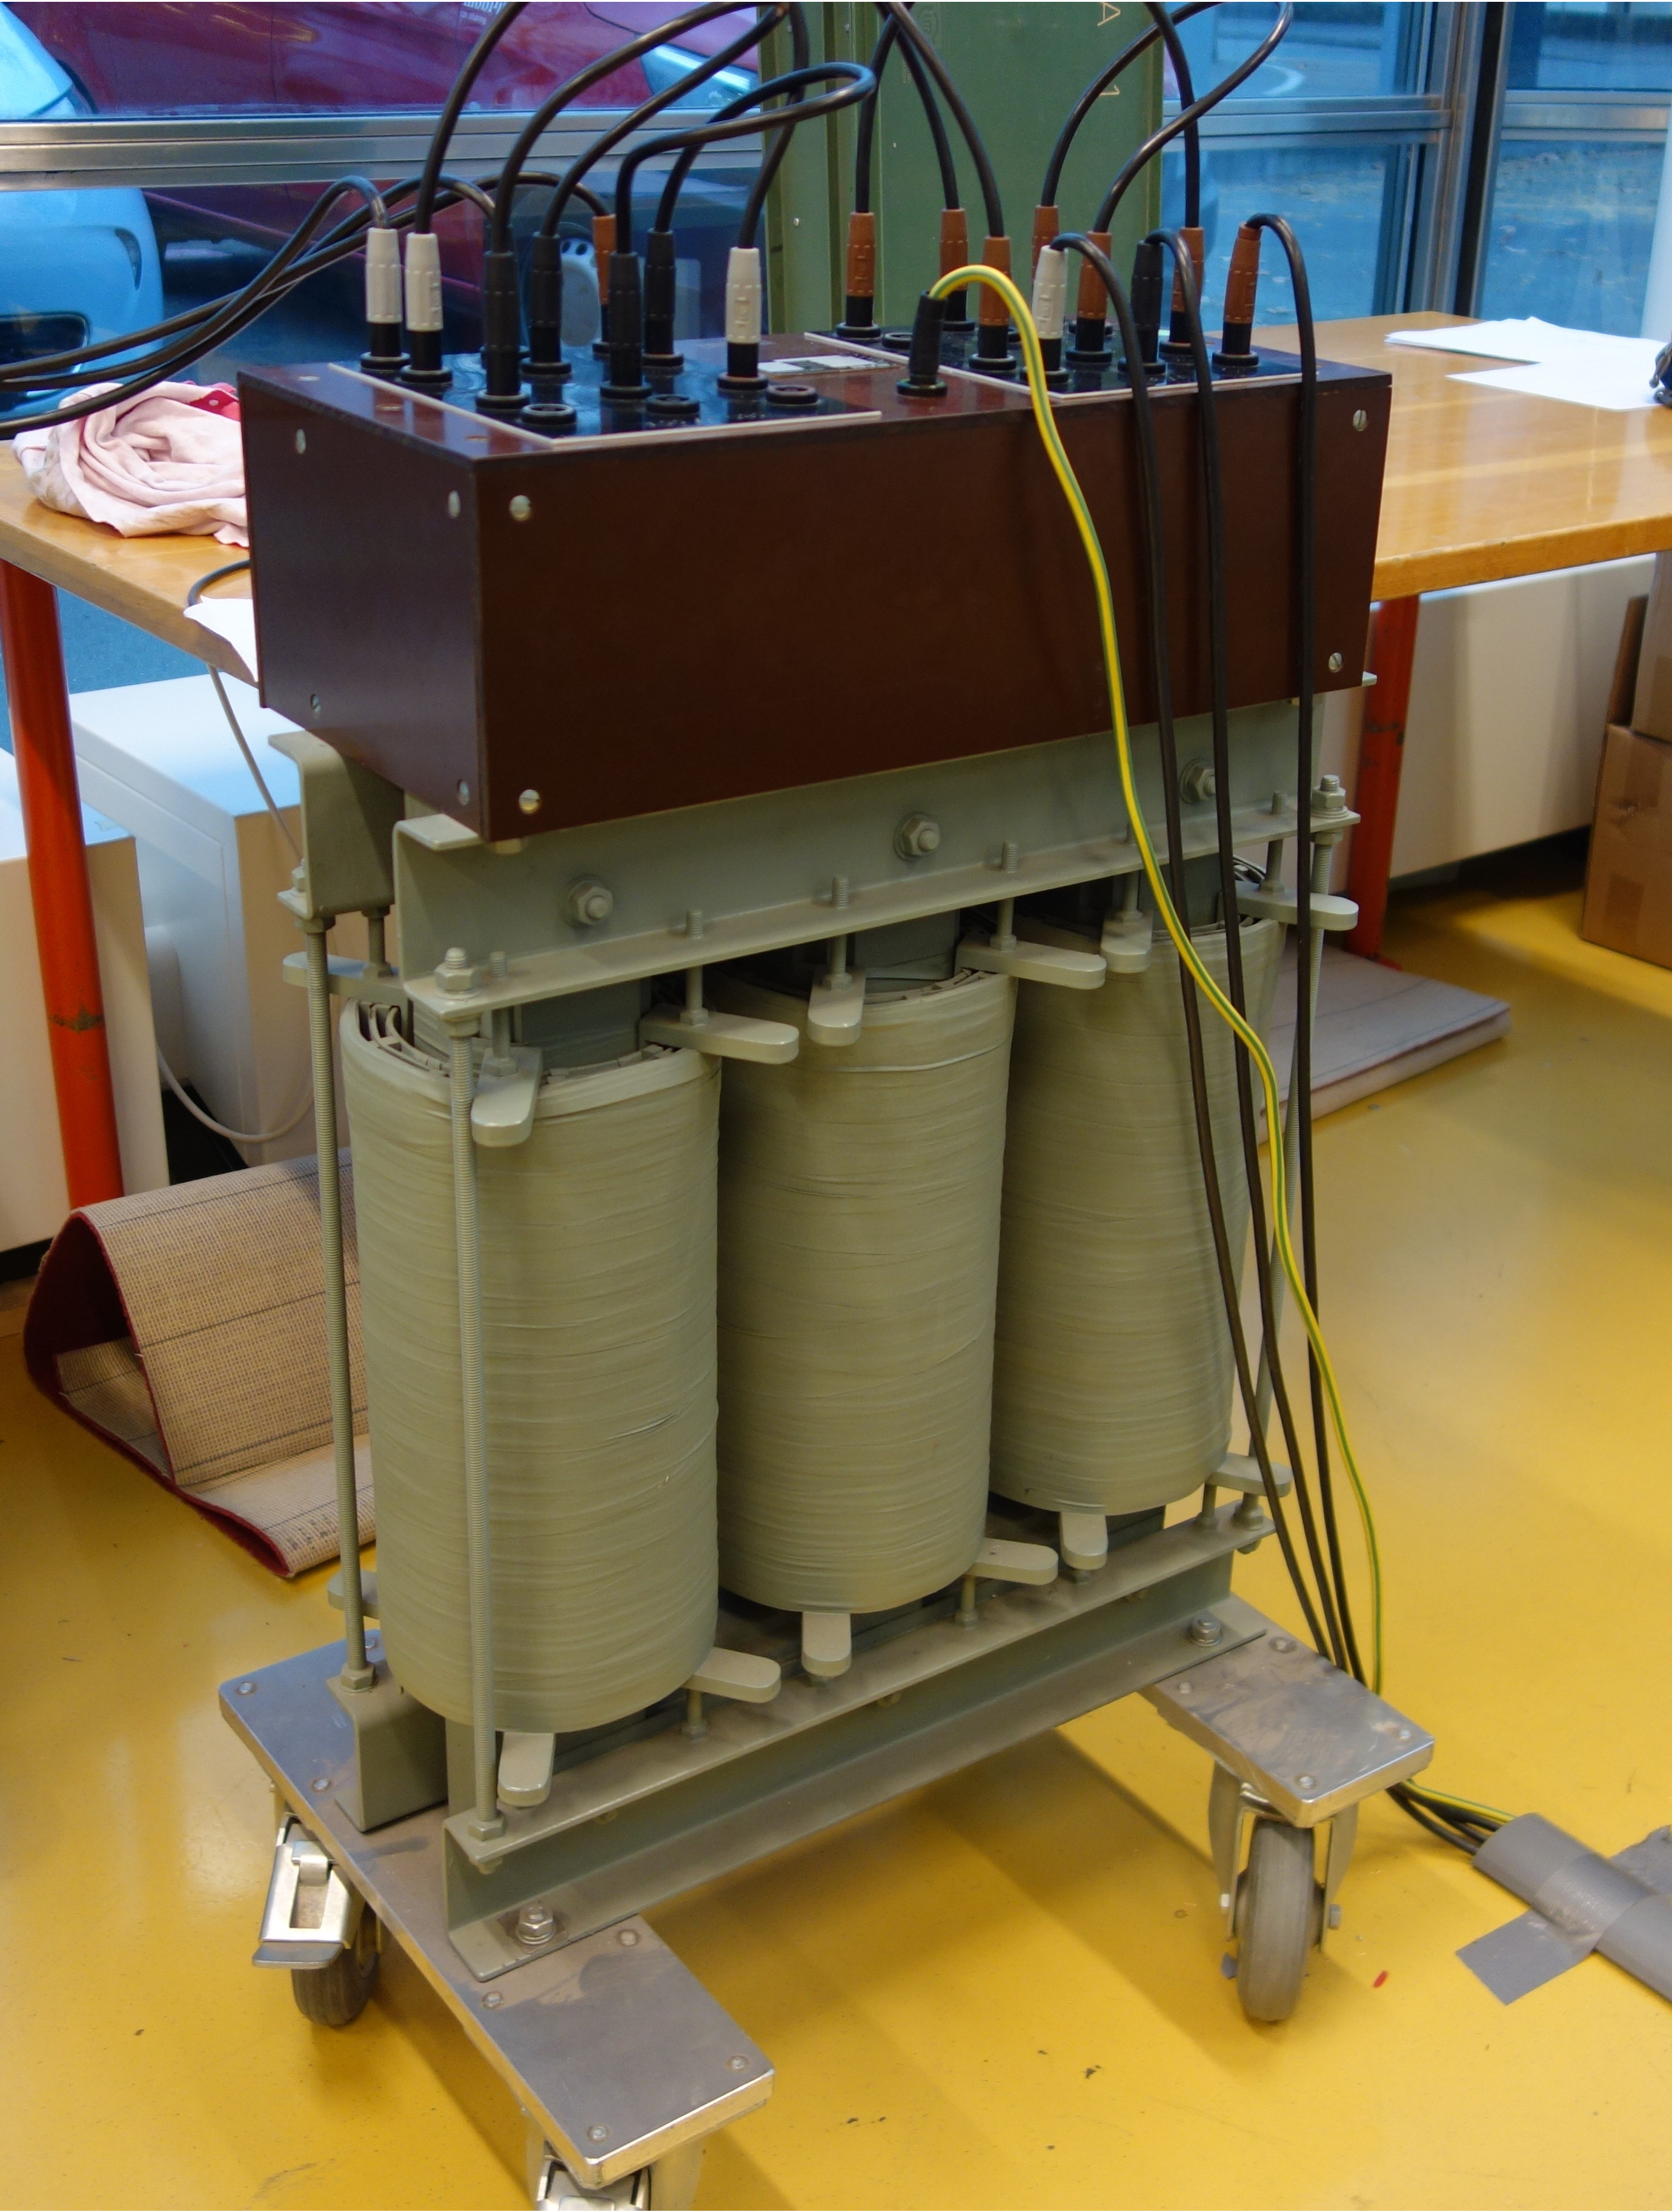
\includegraphics[height=80mm]{Versuchsaufbau/DSC00556.jpg}
		\caption[Transformator Versuchsaufbau]{Transformator Versuchsaufbau}
		\label{fig:Trafo}
	\end{center}
\end{figure}

Der Anschluss erfolgte Primärseitig und Sekundärseitig in Dreieckschaltung und hat einen sekundären Maximalstrom von $95A_{AC}$ bei $127V_{AC}$. Die Gleichrichtung erfolgt mittels einer B-6 Brücke, welche während diesem Projekt selber entwickelt wurde. Der Aufbau ist in nachfolgender Abbildung ersichtlich.

\begin{figure}[H]
	\begin{center}
		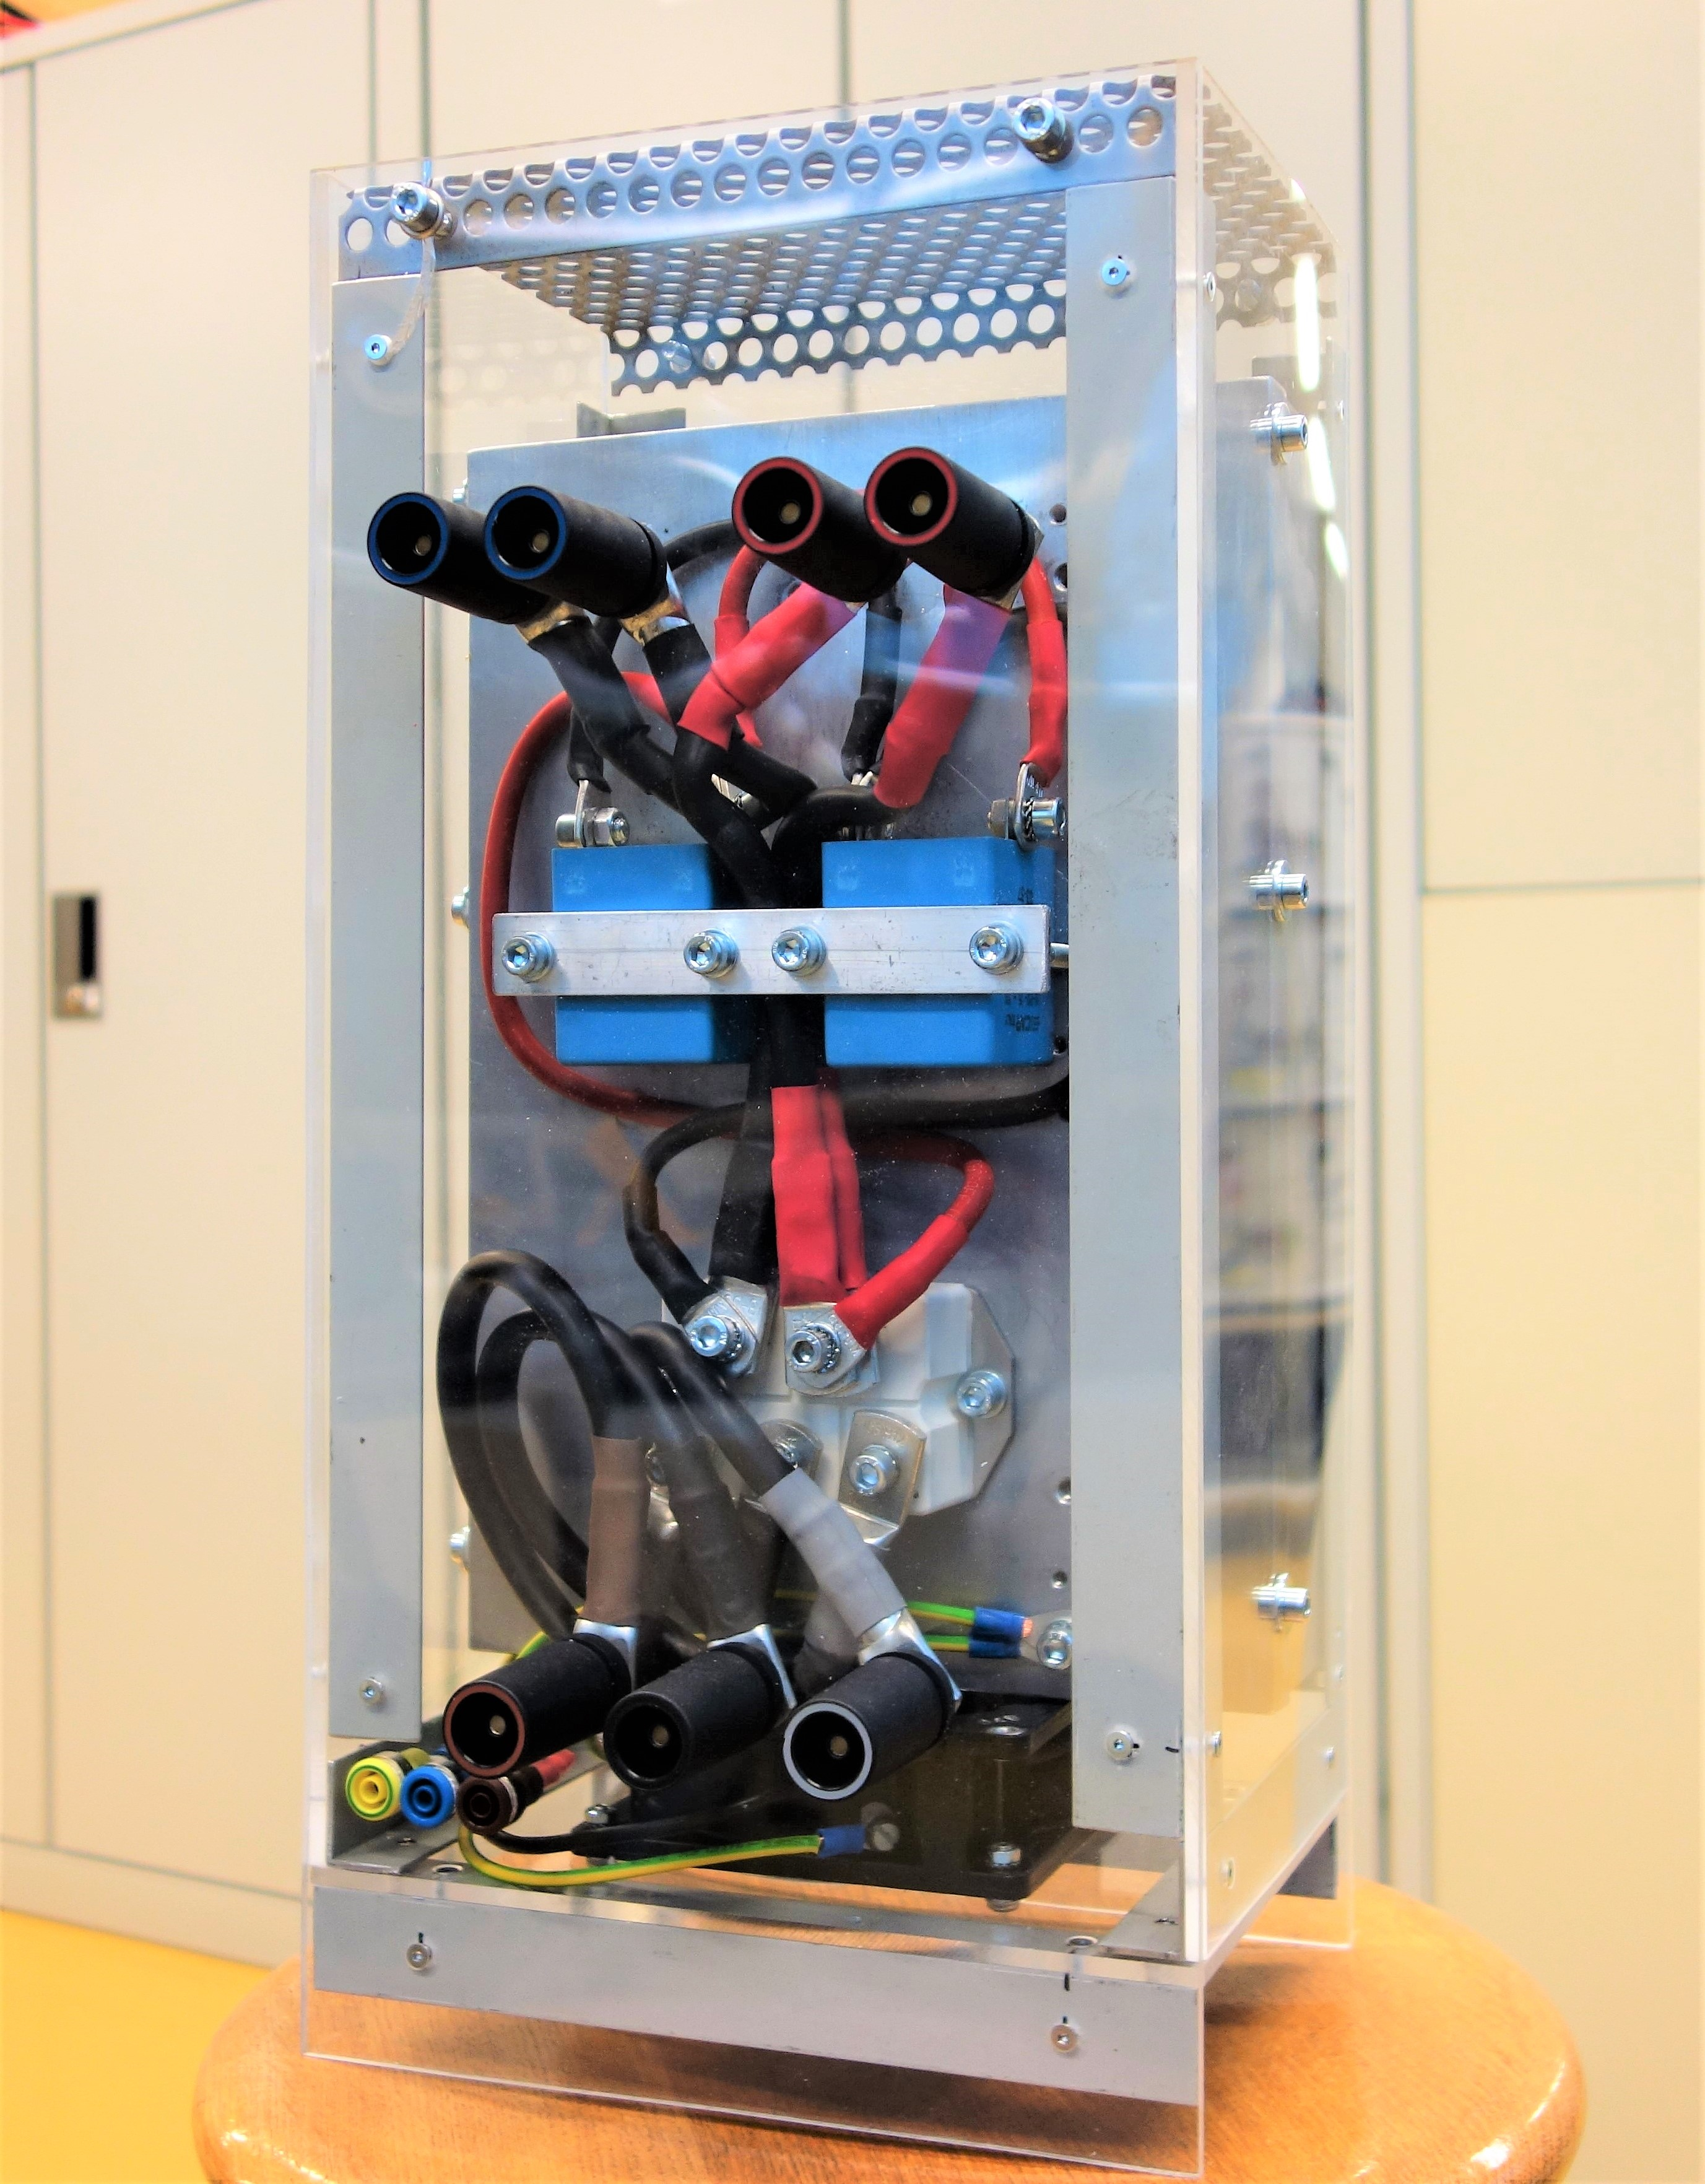
\includegraphics[height=80mm]{Versuchsaufbau/DSC00547(2).jpg}
		\caption[B-6 Gleichrichter]{B-6 Gleichrichter}
		\label{fig:B-6}
	\end{center}
\end{figure}

Die AC-Einspeisung der B-6 Brücke erfolgt mittels den drei Klemmen (Braun, Schwarz, Grau) im unteren Bereich. Diese werden auf den eigentlichen Diodengleichrichter (Weiss) und zwei Stützkondensatoren (Blau) geführt.Gemäss der Formel \ref{eq:B6-Id} ergibt sich somit einen maximalen Zwischenkreisstrom auf der DC Seite von $I_{DC}=\frac{95A}{0.8165} =\underline{116.35A}$.
Dieser erhöhte Strom, wird DC-Seitig durch zwei Hin-, und Rückleiter auf den Motorencontroller geführt. Zwei Elektrolytkondensatoren parallel zur Controller Gleichstromversorgung dienen zur Glättung der harmonischen Wellen und zudem als Entladepuffer bei hohen Belastungen. Controller, DC-Relais und Elkos sind in Abbildung \ref{fig:Controller} ersichtlich. Die DC-Einspeisung erfolgt auf dem orangen Relais und parallel dazu auf den schwarzen seriell geschalteten Elkos.

\begin{figure}[H]
	\begin{center}
		\includegraphics[height=80mm]{Versuchsaufbau/DSC00581.jpg}
		\caption[Controller]{Controller}
		\label{fig:Controller}
	\end{center}
\end{figure}

Betrachtet man das DC-Relais etwas genauer, so sind zwei Steuerdrähte (Gelb \& Grün) ersichtlich. Diese dienen zur Freigabe des Relais welche direkt vom Relais selber gesteuert wird. Tritt ein Fehlerfall auf, kann der Controller dadurch selber die Stromversorgung unterbrechen. Etwas schwerer zu erkennen sind die Kontakte auf dem Controller. Dieser besitzt eine Sicherung direkt nach der Einspeisung des +Pols. Weiter ist ein geflechteter Kabelbaum ersichtlich (welcher alle Kabel zur Ansteuerung des Controllers beinhaltet) und die farbigen Anschlusskabel des Motors auf der rechten Seite. Damit der gesamte Aufbau Kurzschlusssicher ist, wurden alle blanken Elemente mit Klebestreifen isoliert und die Controller Einheit mit einer Kiste abgedeckt.

Die Ansteuerung des Controllers wurde mit einem Mikrocontroller realisiert. Für die Vorgabe des Drehmomentes, konnte ein PWM-Signal mittels zwei Drucktastern verändert werden und auf den Controller übergeben werden. Der legte proportional zur Grösse des Signal eine entsprechende Leistung an den Motor. Der Aufbau des Controllers ist nachfolgend aufgelistet.

\begin{figure}[H]
	\begin{center}
		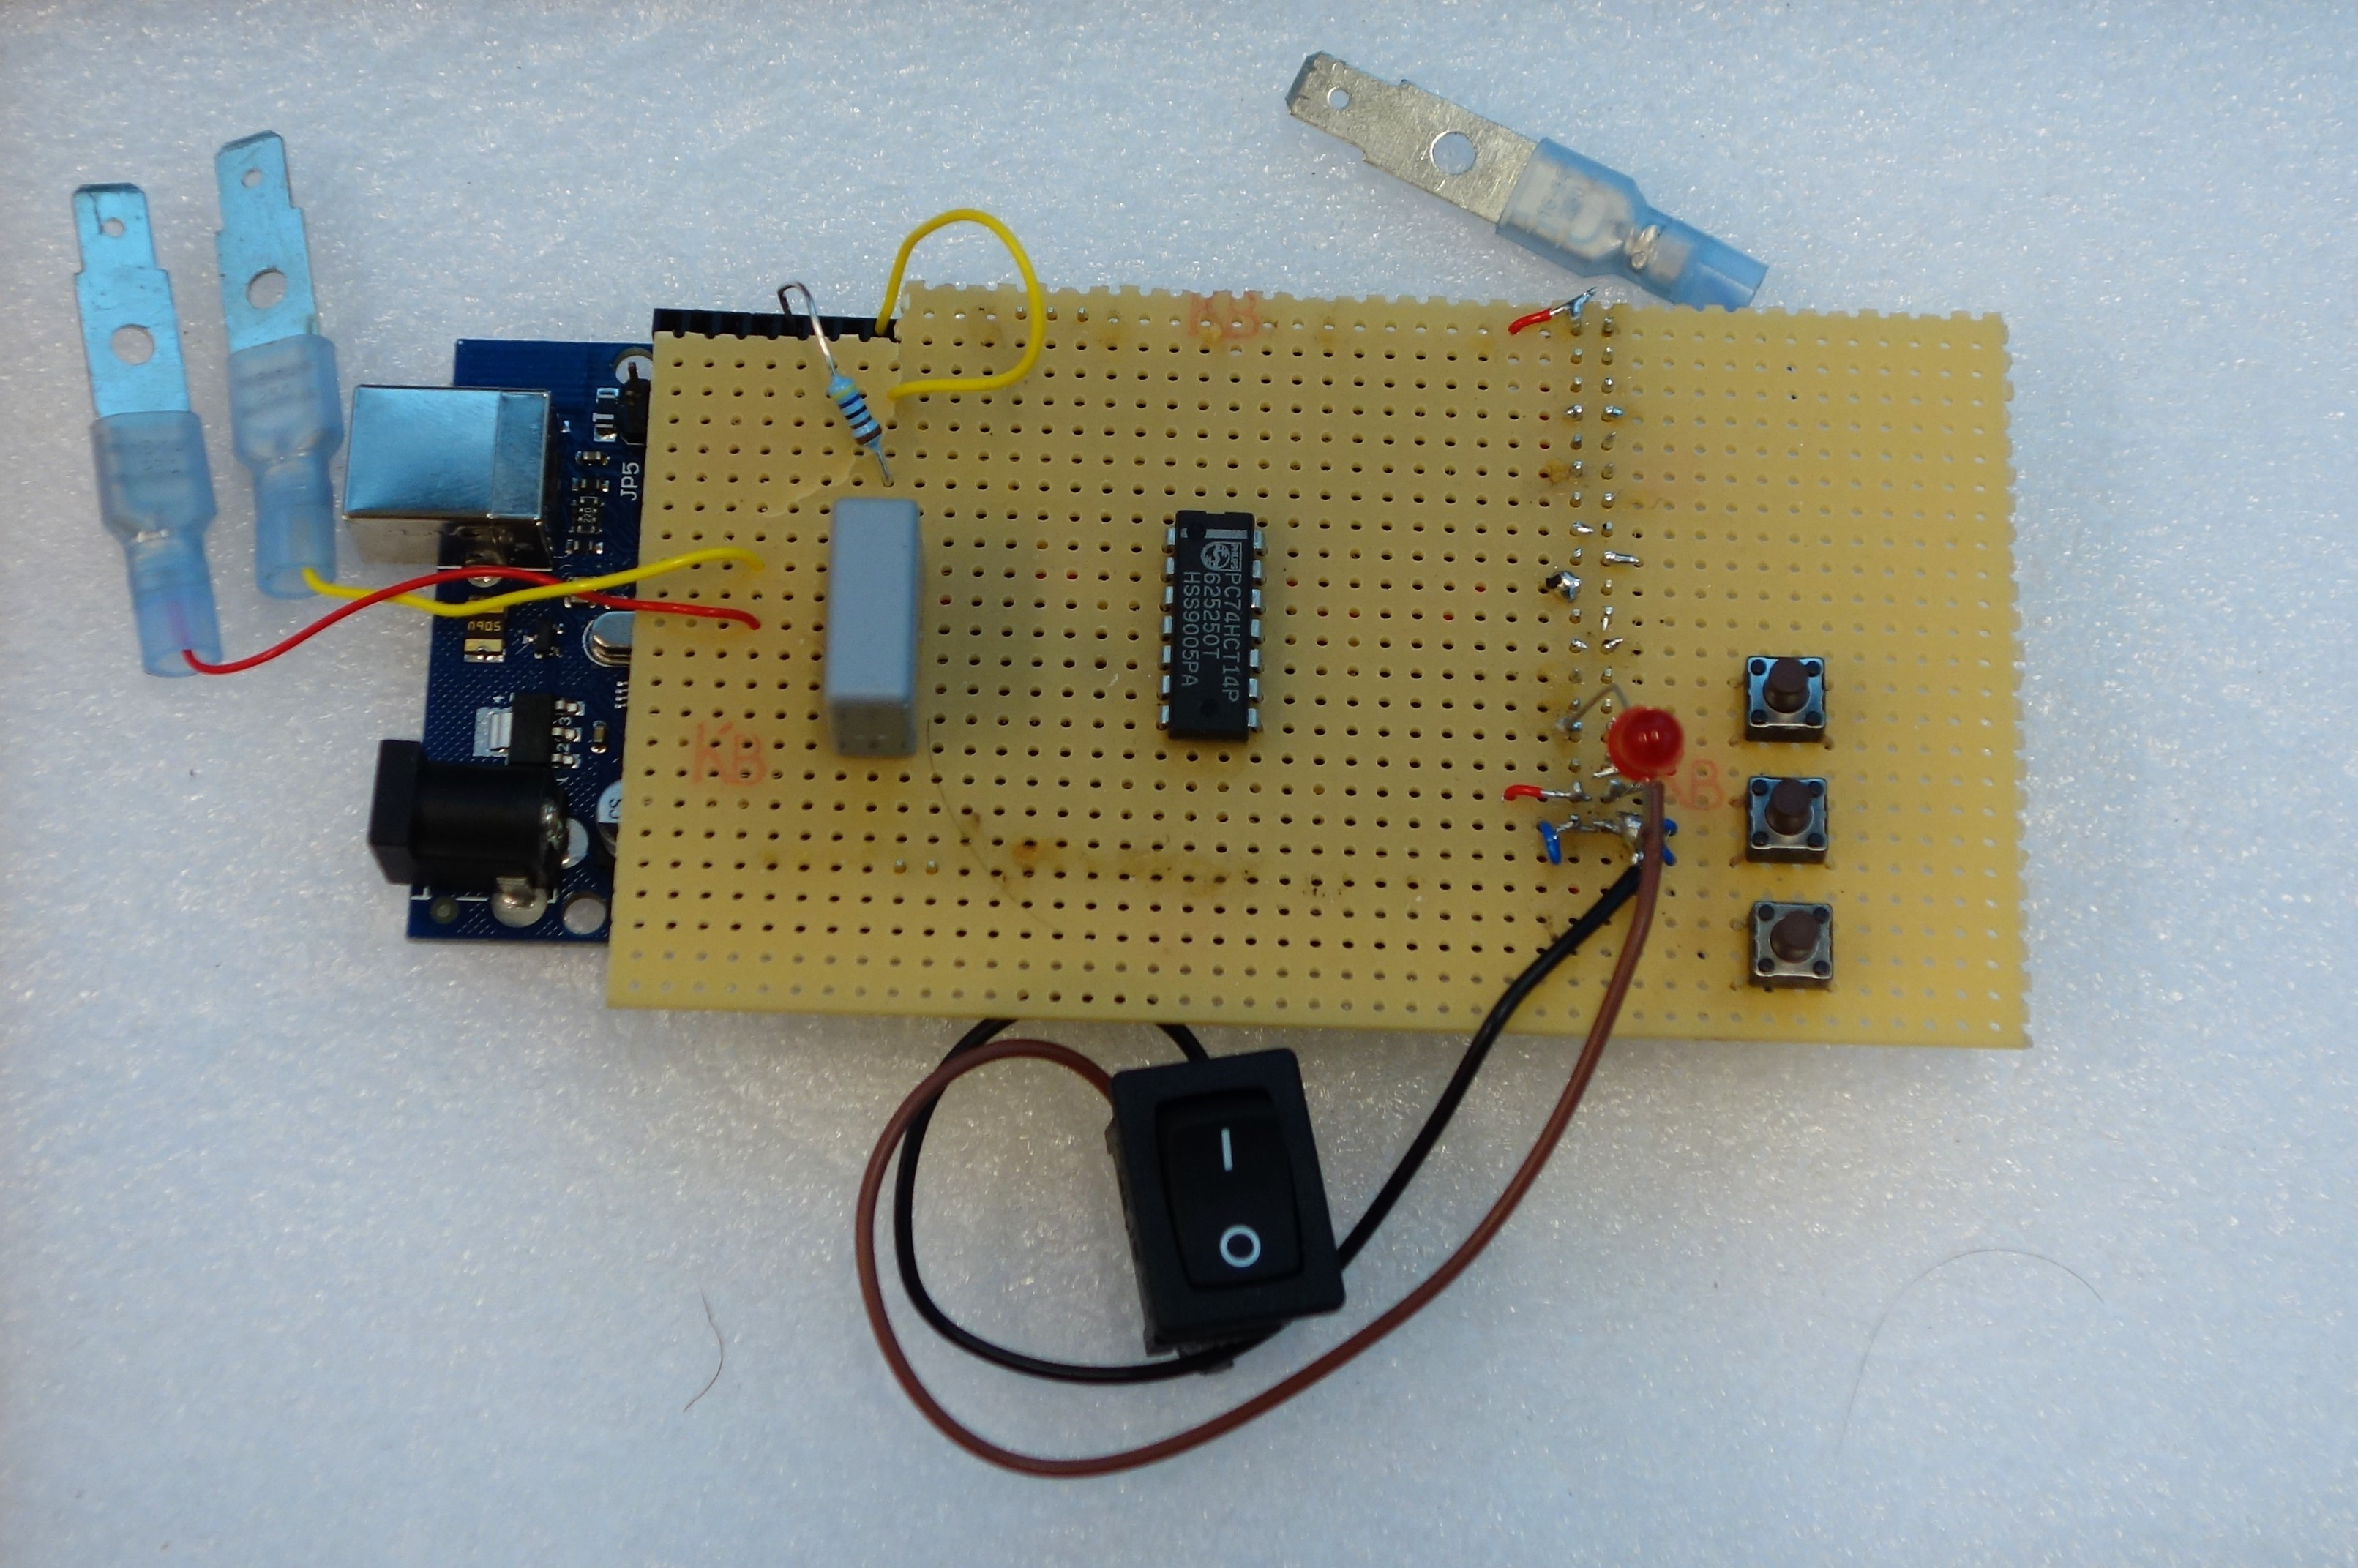
\includegraphics[height=60mm]{Versuchsaufbau/DSC00559.jpg}
		\caption[Controller]{Controller}
		\label{fig:Mikrocontroller}
	\end{center}
\end{figure}
CONTROLLER NOCH GENAUER BESCHREIBEN (Tiefpass, Schnitttriger,...)



Wie anfänglich bereits beschrieben wurde, wurde der verwendete BLDC Motor mit einer ASM gekoppelt. Die Anordnung ist in Abbildung \ref{fig:Motor} dargestellt.
\begin{figure}[H]
	\begin{center}
		\includegraphics[height=100mm]{Versuchsaufbau/DSC00573.jpg}
		\caption[Motor]{Motor}
		\label{fig:Motor}
	\end{center}
\end{figure}
Damit diese zwei Maschinen überhaupt miteinander gekoppelt werden konnten, musste einerseits die Welle des BLDC Motors auf das Niveau der ASM angehoben werden und andererseits seitens der FHNW-Werkstatt einige Anpassungen an der Kupplung getätigt werden. Da der DC-Motor über eine Welle mit Zollmass verfügt, musste eine Kupplung ausgebohrt werden. Weiter verfügt die ASM über keine Nut, weshalb die andere Seite der Kupplung zur Befestigung mit einem Gewinde versehen werden musste. Eine Plexiglasscheibe über der mechanischen Verbindung diente als Berührungsschutz.

Die Ansteuerung der Asynchronmaschine erfolgte mittels eines Frequenzumrichters welcher auf nachfolgendes Abbildung ersichtlich ist.
\begin{figure}[H]
	\begin{center}
		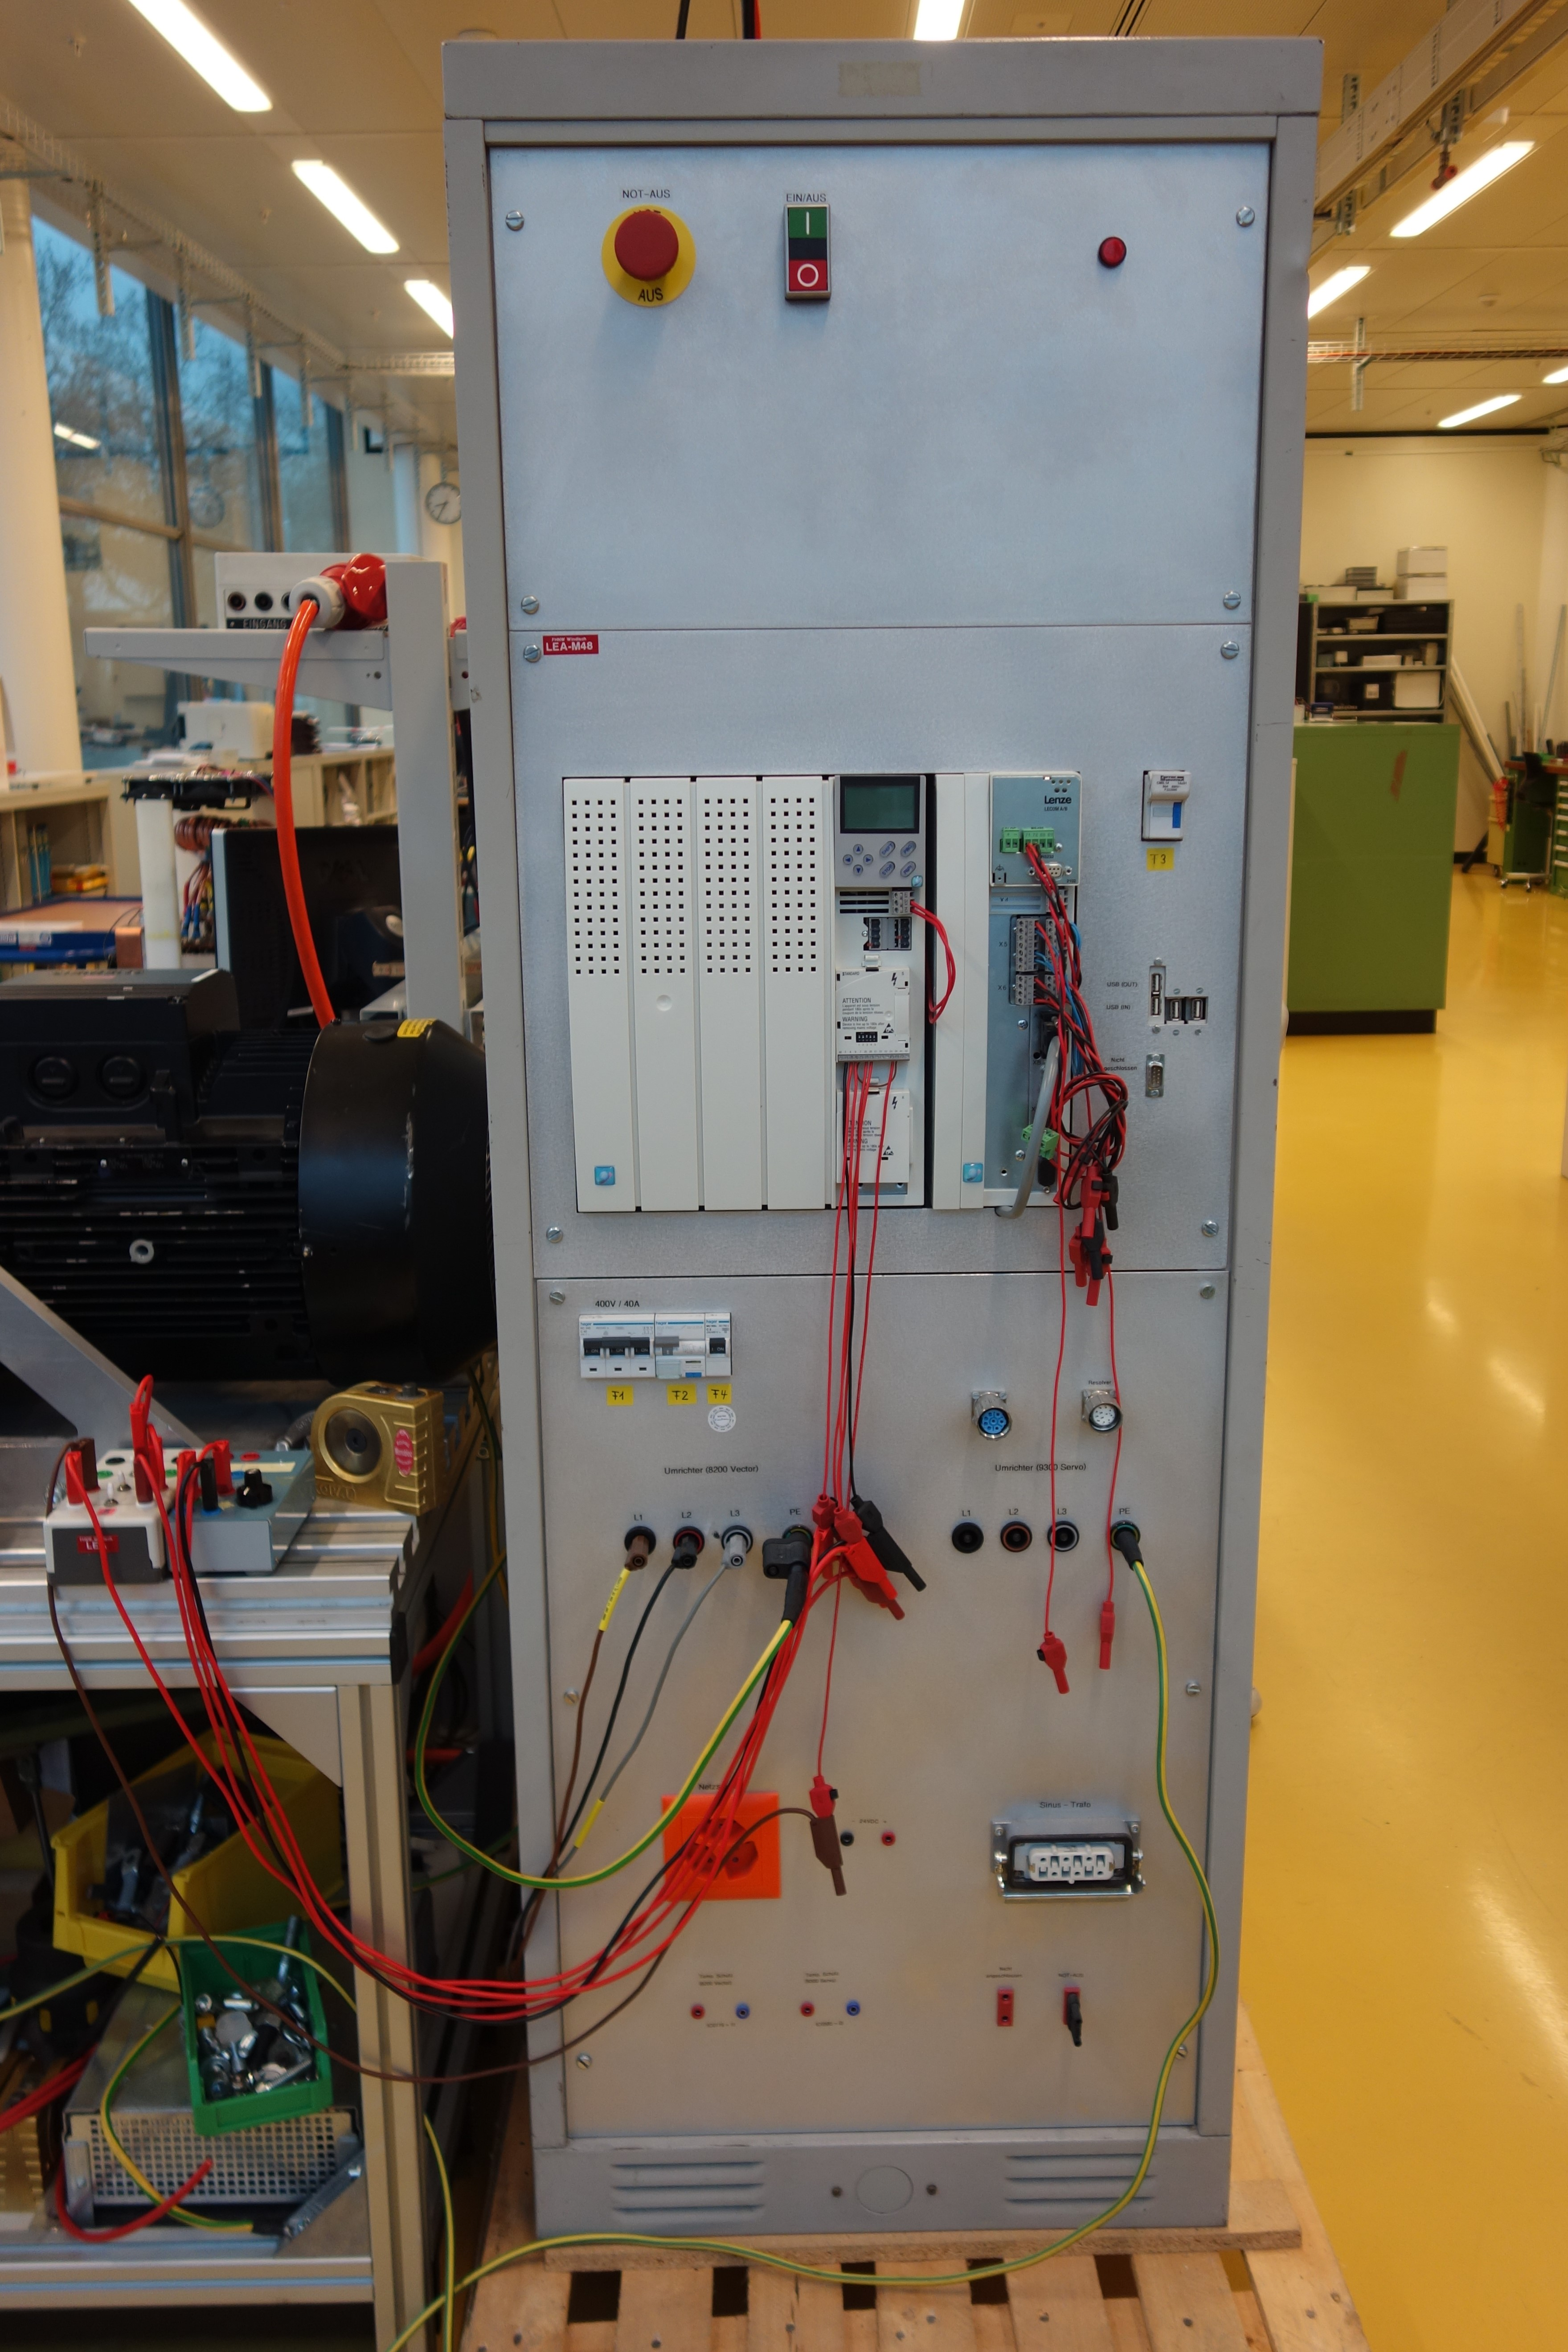
\includegraphics[height=100mm]{Versuchsaufbau/DSC00575.jpg}
		\caption[Frequenzumformer]{Frequenzumformer}
		\label{fig:Frequenzumformer}
	\end{center}
\end{figure}